Для прецизионного детектирования и измерения электронов и фотонов калориметрическая система ATLAS включает в себя электромагнитный калориметр. Он состоит из центрального (баррельного) блока (EMB -- electromagnetic barrel), покрывающего диапазон псевдобыстрот $|\eta| < 1,475$, и пары торцевых частей (EMEC -- electromagnetic end-cap), соответствующих области $1,375 < |\eta| < 3,2$. Электромагнитные калориметры ATLAS построены по гетерогенному принципу, то есть в них разделены функции поглощения и детектирования. В качестве активного вещества служит жидкий аргон, находящийся при температуре около 90K, а для поглощающего материала используется свинец. Между пластинами поглотителя также располагаются медно-каптоновые электроды, по которым происходит снятие сигнала.\par
Заряженная частица, попадая в калориметр, порождает в нём электромагнитный ливень (рис. \ref{fig:em_shower})\parencite{em_shower_wiki}, который детектируется по принципу ионизационной камеры: под воздействием электрического поля между заземлённым поглотителем и электродом, находящимся под высоким напряжением, ионы и электроны дрейфуют, причём последние индуцируют треугольный импульс на электроде (рис. \ref{fig:tri_impulse}) (в действительности, сигнал является более сложным, чем просто треугольник -- в силу поглощения электронов загрязняющими примесями в активном веществе, такими как кислород или хлор, результирующий сигнал падает, а его форма домножается на небольшую экспоненту). Высота индуцированного импульса пропорциональна энергии, накопленной в ячейке калориметра. Время пика импульса используется для определения времени появления частицы.\par
\begin{figure}[ht]
    \centering
    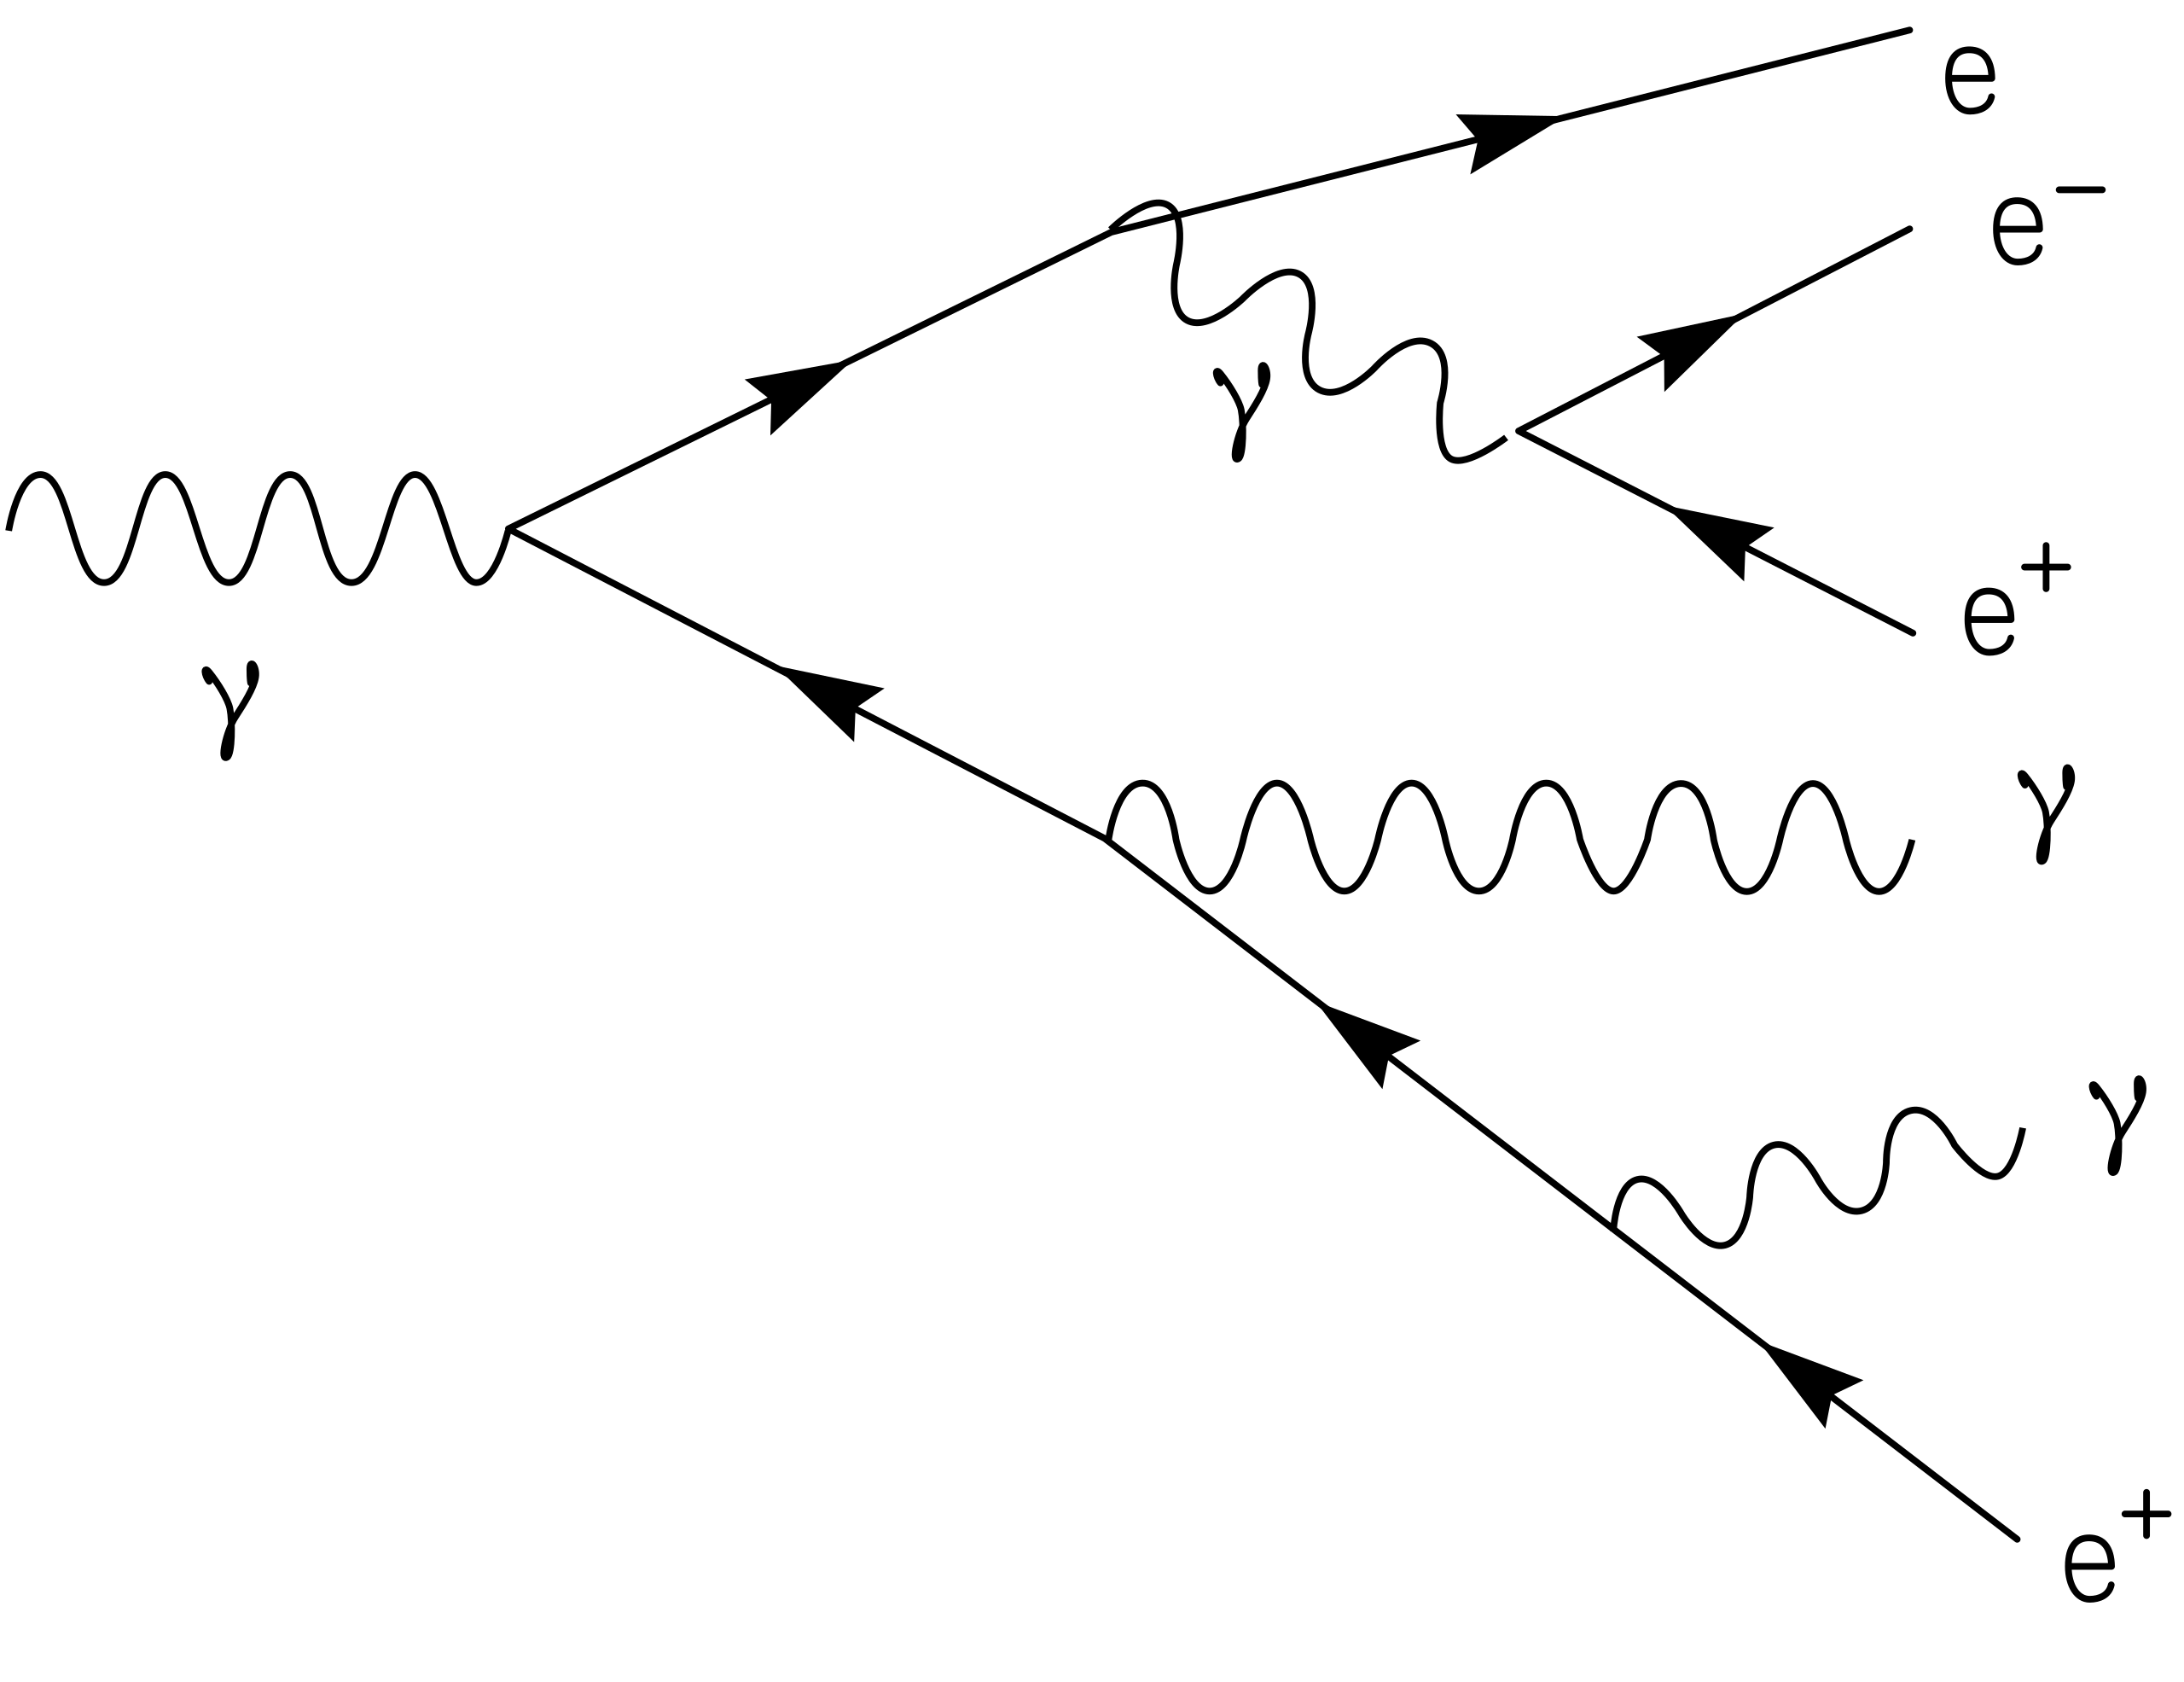
\includegraphics[width=0.5\linewidth]{em_shower.png}
    \caption{Схема электромагнитного ливня}
    \label{fig:em_shower}
\end{figure}
\begin{figure}[ht]
    \centering
    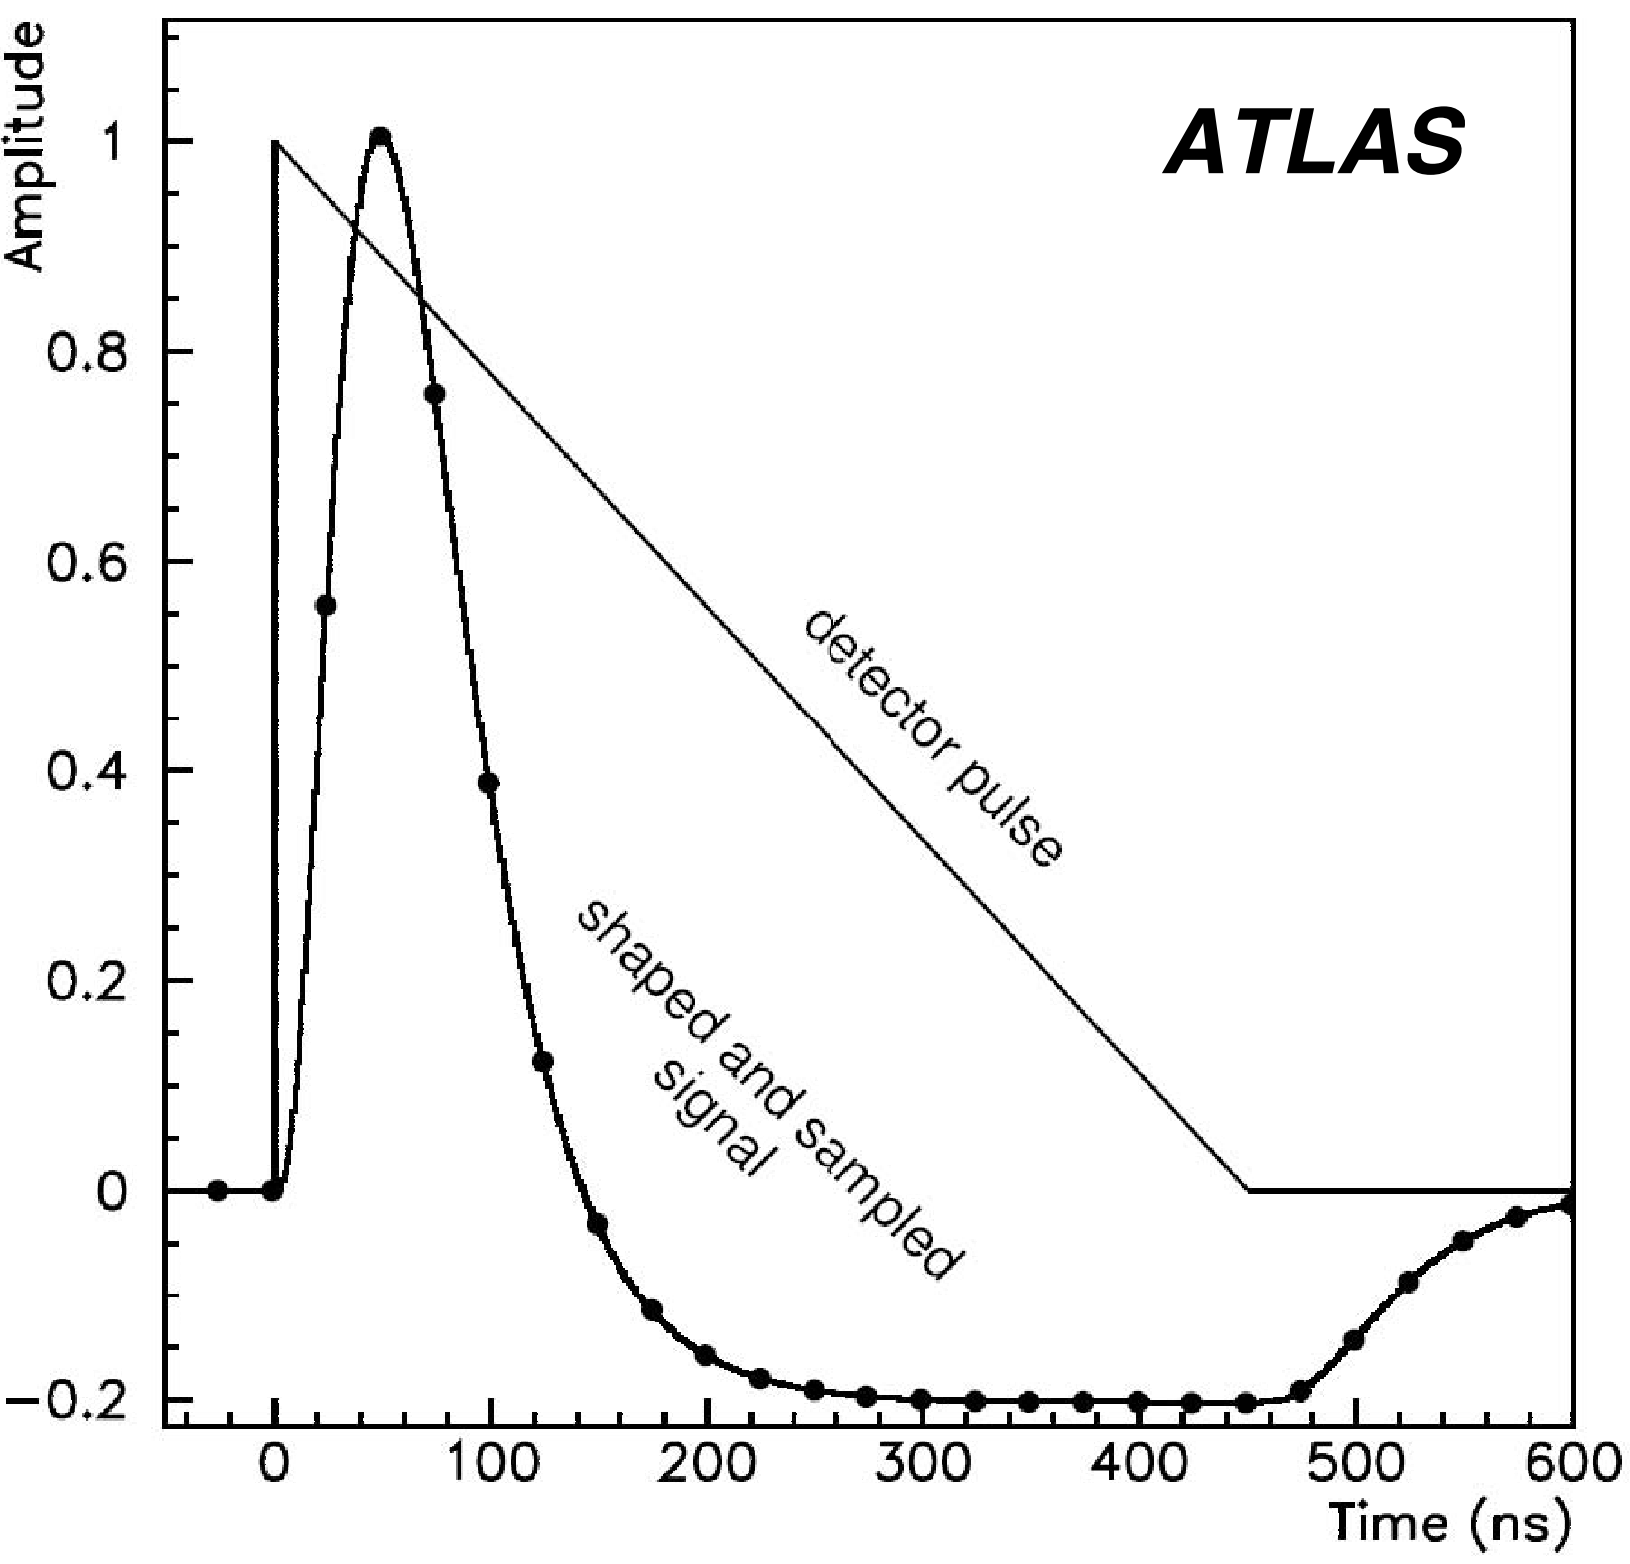
\includegraphics[width=0.5\linewidth]{tri_impulse.png}
    \caption{Форма импульса тока электромагнитного калориметра и выходного сигнала после формирования}
    \label{fig:tri_impulse}
\end{figure}
Электромагнитный калориметр имеет сложную геометрию в форме гармошки (аккордеон). Это позволяет достичь полной симметрии калориметра по азимутальному углу, а также обеспечить высокую гранулированность детектора и увеличить его быстродействие за счёт малого зазора между пластинами. Толщина EMB составляет более 24 радиационных длин ($X_0$, расстояние, на котором интенсивность потока электронов высокой энергии и гамма-излучения падает в e раз). Каждый модуль калориметра имеет ячеистую структуру и поделён на несколько слоёв по глубине, как, например, модуль центрального блока на рис. \ref{fig:em_cal_struct}. Калориметр сконструирован так, что наибольшая часть энергии собирается в среднем слое, задний слой собирает лишь хвост электромагнитного потока. Передний слой сегментирован таким образом, чтобы с его помощью можно было максимально точно определить направление падающих частиц. Исходя из этого, используя измерение энергии и положения всех ячеек в каждом слое калориметра можно восстановить энергию и траекторию рождённых частиц.
\begin{figure}[ht]
    \centering
    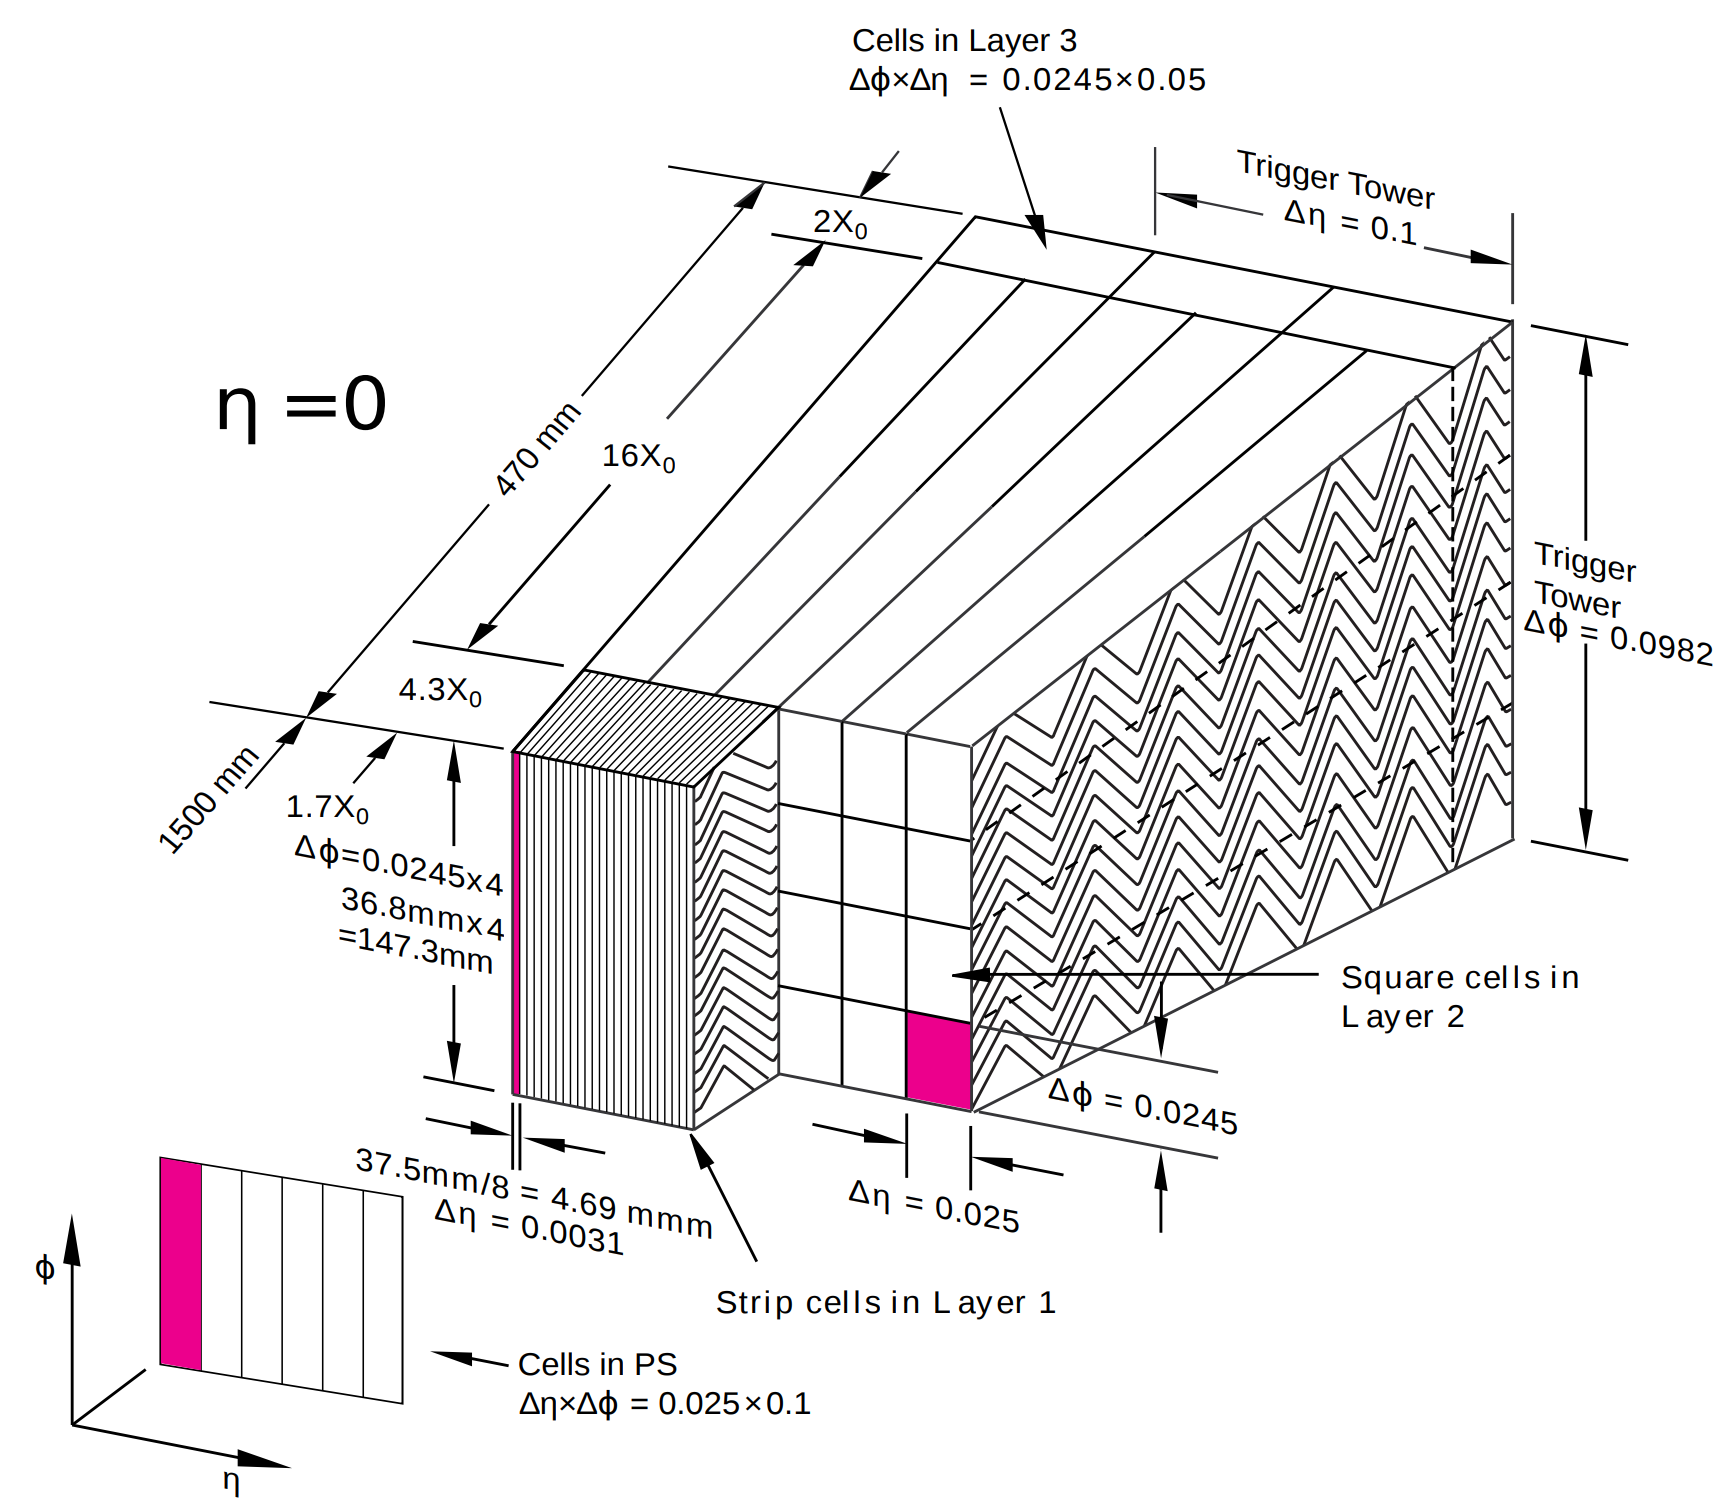
\includegraphics[width=0.7\linewidth]{em_cal_struct.png}
    \caption{Схема разделения модуля EMB по слоям}
    \label{fig:em_cal_struct}
\end{figure}
